\documentclass{article}

\usepackage{tikz}

\begin{document}

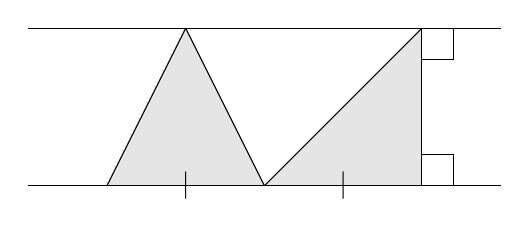
\begin{tikzpicture}
  \fill [color=gray!20] (0,0) -- (2,0) -- (1,2) -- cycle;
  \fill [color=gray!20] (2,0) -- (4,0) -- (4,2) -- cycle;
  \draw (1,2)-- (0,0);
  \draw (2,0)-- (1,2);
  \draw (4,2)-- (2,0);
  \draw (4,0)-- (4,2);
  \draw (-1,0)-- (5,0);
  \draw (-1,2)-- (5,2);
  \draw(1,0) node{$|$};
  \draw(3,0) node{$|$};
  \draw  (4,1.6)-- (4.4,1.6);
  \draw  (4.4,1.6)-- (4.4,2);
  \draw  (4.4,0)-- (4.4,0.4);
  \draw  (4.4,0.4)-- (4,0.4);
\end{tikzpicture}

\end{document}
